\chapter{1. Introduction}

\section{Overview}

Technology and its products influence public norms, which then will affect tools; both have a mutual dependence. This thesis positions a novel tool for civic engagement within this loop of society and technology influencing each other. \hlcyan{Mechanisms that work with the combination of technology and societies are sociotechnical systems.{\cite{bruno1992missing}} \footnote{
Bruno puts the goal of socialtechnical study is:
{\tiny
\begin{quotation}
to follow the dynamic of reinscription
transforming a silent artifact into a \textit{polemical} process.
\end{quotation}
}
}}

\begin{figure}[!htb]
 	
\includegraphics[width=\textwidth]{chapters/1/fig/hearings.png}               
 	 \caption[diagram: community hearings]{The pyramid divided into two parts; The top portion includes the Planners, Governors, and Stakeholders, and the rest. The diagram shows one typical procedure known as public meetings which is a communication tool to let the top gain feedback from the bottom. The arrow pointing to the black border indicates it changes the infrastructure, which is the border of the built environment and the natural environment.
}
  	\label{fig:hearings}
\end{figure}

Traditionally the urban planning process accommodates public feedback through public meetings for voicing concerns from the community. \hlcyan{Opening a public meeting is perhaps the most basic and dominant method of today's public engagement method used in urban planning.} The planners, government, and stakeholders will interpret the input, and plan and execute interventions that consider citizens' feedback. We can think of this as a necessity to accommodate feedback once cities become too large for governance via a direct democratic approach.
\begin{figure}[!htb]
 	
\includegraphics[width=\textwidth]{chapters/1/fig/community_engagement.png}               
 	 \caption[externalized proposal]{\protect\raggedright Demand from both the planners (wicked problem \cite{churchman1967guest}) and the community (evidence of urbanization leads to democratization \cite{woolley2010evidence})to externalize the proposal (rectangle with P). Now citizens can provide feedback and co-design the interventions. This
is the typical diagram for today's community engagement. The planners are still proposing the plans which are the primary generator of solutions.
}
  	\label{fig:spin_margin}
\end{figure}
Urbanization occurs and as cities increase their density, public demand for transparent planning also rises, having the proposal to be externalized for scrutiny by the community. This high demand, especially for transportation planning, indicates the opportunity for new tools to better serve public needs.

In addition, new tools that leverage pervasive mobile communications have been developed to collect data in the form of reports and claims. These applications can be categorized as `structured' / `unstructured'. The majority of these applications solicit unstructured feedback, making them useful for general comments, but limiting their utility for actionable information.

These tools are mainly used for analyzing the current situation, distinct from integrating (synthesis) it to one executable plan. Designers and architects who have been generating 
actionable interventions, have been continuously arguing that the process of analysis and synthesis should be as close as possible in order to be designed properly. The absence of the synthetic phase mainly comes from the difference in objective because the designers' and architects' main goal is the integration of a plan, \hlcyan{which is beyond collecting data and interpret it}. The disjoint of analysis and synthesis is one reason for failing design, since both, as well as the bond between them, are essential to the feedback process. Yet the synthetic process in planning required domain knowledge, was difficult, and notably slow, the community had limited exposure to this step of \textit{the realization of the program}. Thus, today's community engagement processes do not have a clear distinction between the two major phases of design.

The evolution of technological tools for urban planning and their relationship to public demands will be explored \hlcyan{in Chapter 2}.

\begin{figure}[!htb]
 	
\includegraphics[width=\textwidth]{chapters/1/fig/cityscope.png}               
 	 \caption[diagram: cityscope model]
 	 {\protect \raggedright The cityscope model covers the analysis through the prioritization phase. Apart from the visualization and tangible interface, it is a tool for
 	 iterating the analytic phase and synthetic phase. Note the arrow from Planners to the Plan is approval, which the plan generation is a collective collaboration from the whole community. \cite{moe2016illuminate}}
  	\label{fig:diagram_cityscope}
\end{figure}

New tools are also fragmented, focusing to support specific parts of the process. As these tools become sophisticated, there is potential to have them as an integrated system that provides easy transition between the analytic and synthetic phases, thus a faster iteration of trial and error. \hlcyan{A list of tools is provided in Chapter 3 to discuss different attempts of community engagement.}

This thesis looks at a specific topic in urban planning: making cities more accessible to bicycles. The tool - bikebump - that allows users to passively report problems with urban infrastructure, then invites them to actively participate in planning processes to improve the urban environment. Having an integrated platform though the data collection and plan proposal is what makes this attempt novel.


\begin{figure}[!htb]
 	
\includegraphics[width=\textwidth]{chapters/1/fig/bikebump.png}               
 	 \caption[diagram: bikebump]{This thesis proposes and implements an integrated tool that prioritizes contextualized data collection used for urban planning interventions.}
  	\label{fig:diagram_bikebump}
\end{figure}

% \begin{figure*}[!htb]
% 
\includegraphics[width=\textwidth]{chapters/1/fig/proposed_process.png}               
%  	 \caption[proposed method]{The proposed method using bikebump trying to fit the current system. The Transportation
% Improvement Program (TIP) is a federal requirement for each state to compile
% a list of executable improvements regarding transportation issues. The top of the pyramid from the previous includes the Metropolitan Planning
% Organization and the Mayor (city CEO), given a roll of approval (which is no different from another single vote) and metric modification and engineering
% of plans. The improvement plans that was generated and prioritized by bikebump will undergo one last process of being approved by the
% Transportation Advisory Council which also tied to a public hearing.
% }
%   	\label{fig:proposed}
% \end{figure*}

Chapter 4 will look into implementation; not only the actual development of the tool, but a schematic of how this approach may be integrated into the real situation. 
\hlcyan{This proposed method has two major differences compared to the method that is currently conducted through the United States.} One, the box has inputs in two different directions from the community, indicating the data analysis and plan synthesis. Two, the planners\footnote{Metropolitan Planning Organization} and the mayor\footnote{sometimes referred as the city CEO} will have a different type of \hlcyan{role} when it comes to approving and modifying the metrics to align with the long running plans. The chapter will cover the comparison of the current standard process, with the tools and methods used for developing this web-based application, and the procedure of how it will work. It will also cover the  experiment conducted to see the application's performance. Figure \ref{fig:how} shows the procedure of the user experience. 
\begin{enumerate}
    \item User rings the bell if there is something worth reporting (a DING). Simple protocol of single DING indicating ``unsafe/dangerous'' and double DING indicating ``safe/pleasant''
    \item Smart phone detecting the bell sound from pre-calibrated frequency \footnote{The application has access to the phone's microphone and can detect the ring, saving a short sound clip of the moment before the bell ring. }
    \item Geolocation, ``dangerous/pleasant'' value, and sound clip sent to database
    \item The data will be mapped to a web browser interface that others would be able to observe.
    \item User provides complementary information about the DING.
    \item User propose an improvement plans by selecting a solution and the road.
    \item User votes for improvement plans the agree to have.
\end{enumerate}
\begin{figure}[!htb]
    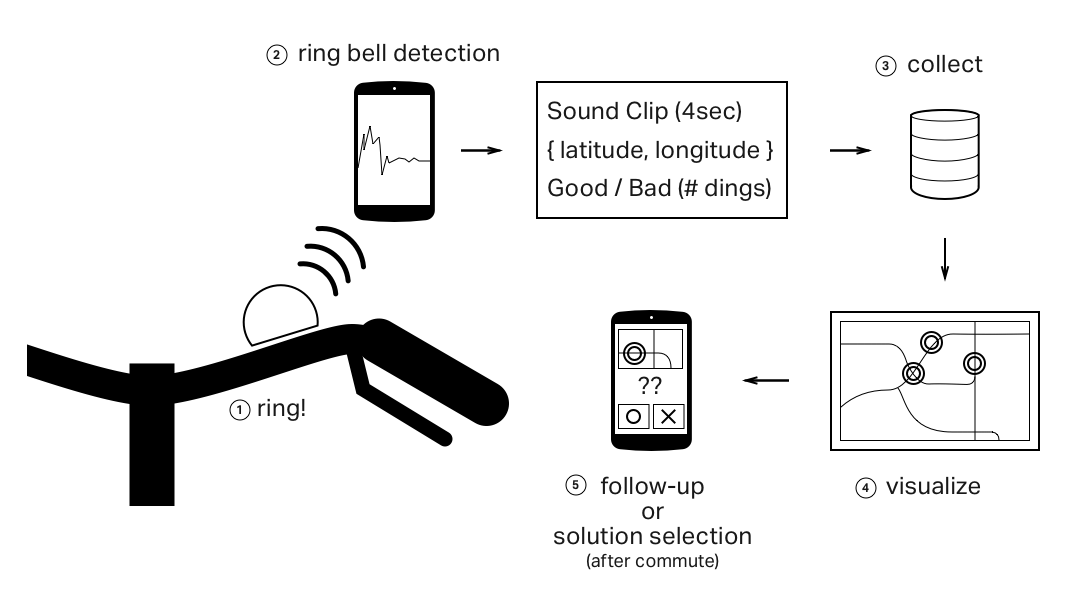
\includegraphics[width=\textwidth]{chapters/1/fig/how_it_works.png}               
    \caption[how bike bump works]{
        The flow of user interaction. 1.user rings bell 2.smart phone detects bell 3.data sent to server 4.visualized onto Map 5. followup questions, proposing improvement plans, and voting.
    }
    \label{fig:how}
\end{figure}
\section{Contribution}
The main contributions of the thesis are to connect citizens into the urban planning process through a novel technological
solution. By harnessing feedback from individual bicyclists, the the tool opens the urban planning process
beyond mayors, professional planners and includes average citizens \hlcyan{who can collectively architect} the physical
environment surrounding use. It may also help the planning side to understand the residents' demands.
In addition, the schema for the new urban planning support tool will externalize the process plan analysis and synthesis,
which is often tacit knowledge within the planners. The study proposes a bi-directional communication
method to connect the top and bottom of the process.
